\chapter{Dojo diagram package}

\section{Overview}
	\begin{figure}[ht]
			\begin{center}
				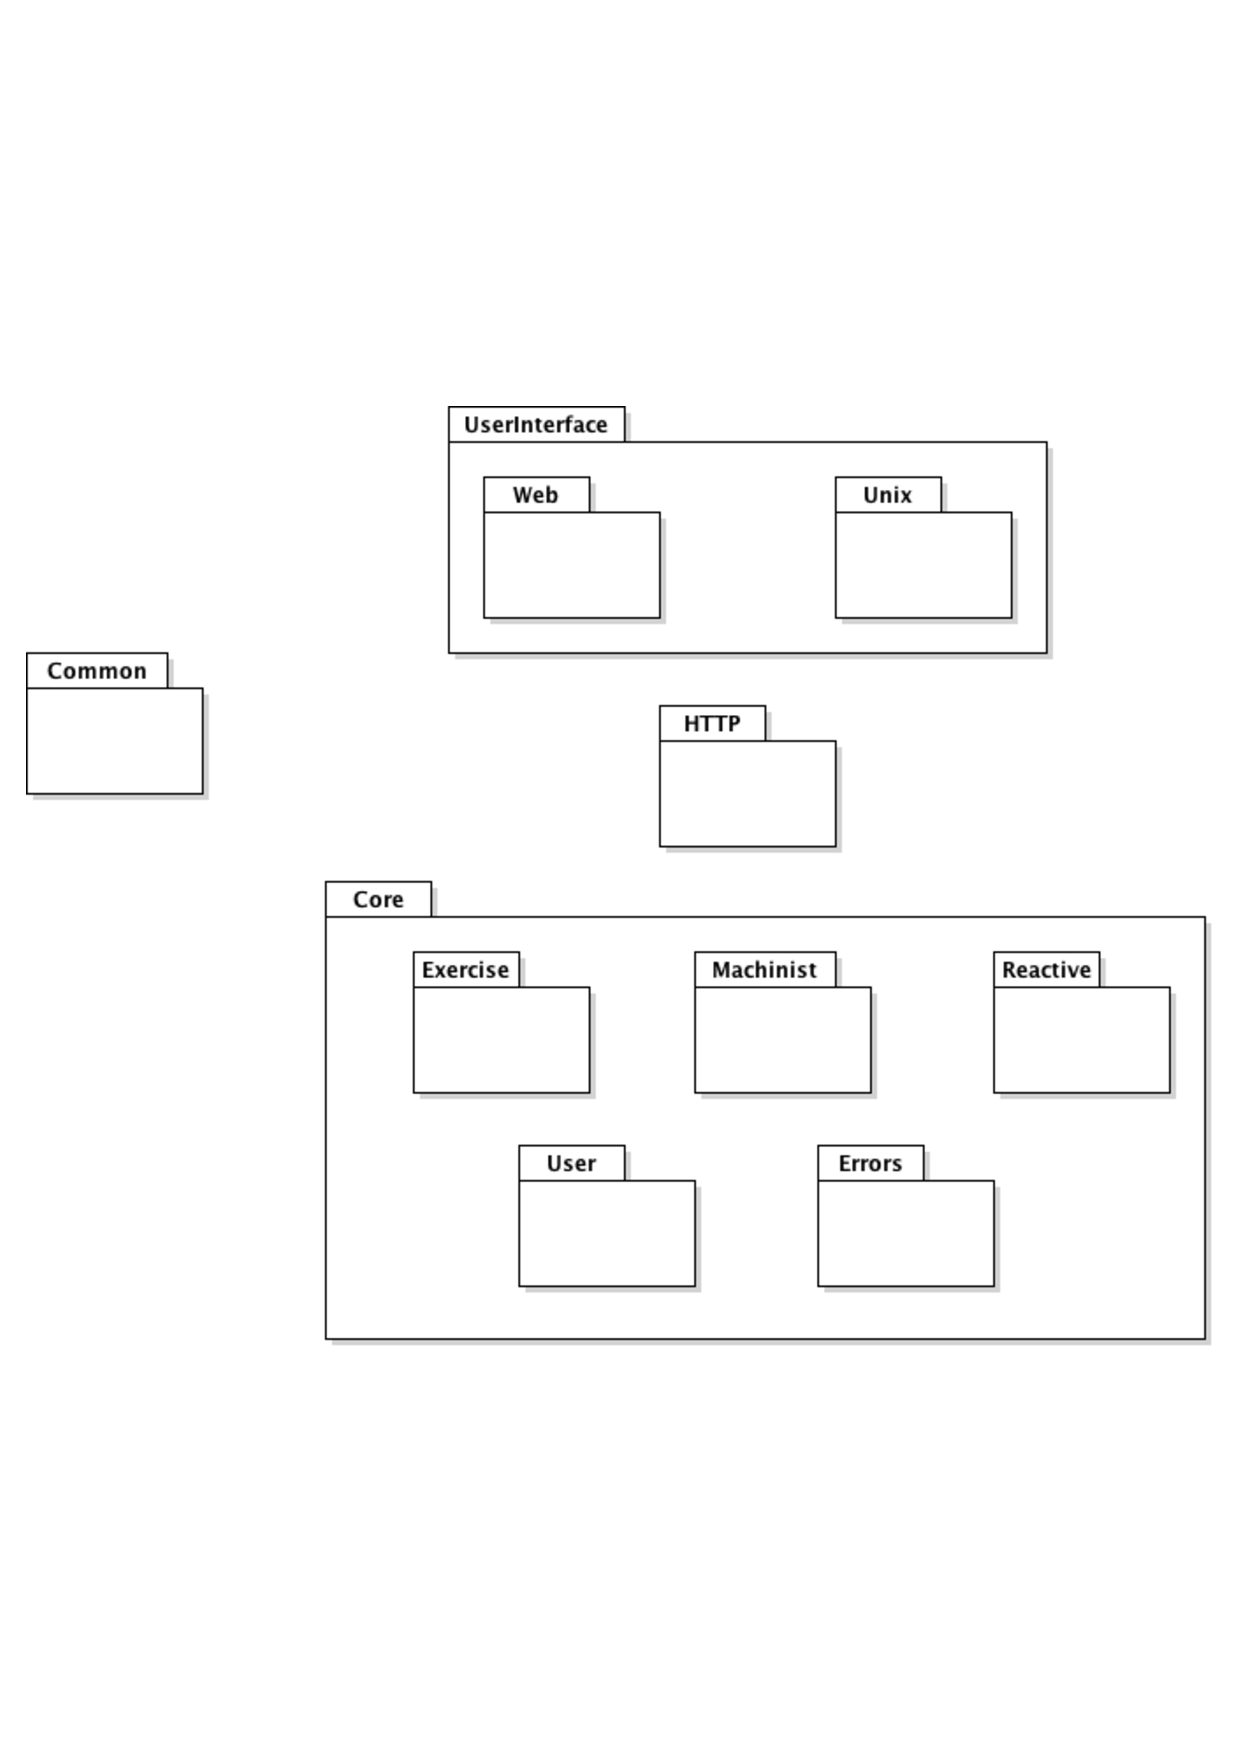
\includegraphics[width=\textwidth,  trim=2cm 6cm 2cm 7cm]{UML_figure/DP/general/DP_General.pdf}
				\caption{Diagram package : Overview}
			\end{center}
	\end{figure}
	\section{User Interface}
		This package holds every interface for the user.
		\subsection{Web}
			This package holds units which define the Web Interface
		\subsection{Unix}
			This package holds units which define a Shell Interface for Unix user.
	\section{HTTP}
		This package holds the web services which allow the user interface to communicate with the core.
	\section{Core}
		This package holds the logical platform units.
		\subsection{Exercise}
			This package holds units which define exercise entities.
		\subsection{Machinist}
			This package holds units which define machinist entities.
		\subsection{Reactive}
			This package holds units which define reactive entities.
		\subsection{User}
			This package holds units which define user entities.
		\subsection{Client}
			This package holds units which define client.
		\subsection{Errors}
			This package holds units which define errors entities.
	\section{Common}
		This package holds every units which are used in each package.
%end chapter diagram package
